\documentclass[]{book}
\usepackage{lmodern}
\usepackage{amssymb,amsmath}
\usepackage{ifxetex,ifluatex}
\usepackage{fixltx2e} % provides \textsubscript
\ifnum 0\ifxetex 1\fi\ifluatex 1\fi=0 % if pdftex
  \usepackage[T1]{fontenc}
  \usepackage[utf8]{inputenc}
\else % if luatex or xelatex
  \ifxetex
    \usepackage{mathspec}
  \else
    \usepackage{fontspec}
  \fi
  \defaultfontfeatures{Ligatures=TeX,Scale=MatchLowercase}
\fi
% use upquote if available, for straight quotes in verbatim environments
\IfFileExists{upquote.sty}{\usepackage{upquote}}{}
% use microtype if available
\IfFileExists{microtype.sty}{%
\usepackage{microtype}
\UseMicrotypeSet[protrusion]{basicmath} % disable protrusion for tt fonts
}{}
\usepackage[margin=1in]{geometry}
\usepackage{hyperref}
\hypersetup{unicode=true,
            pdftitle={Streamline Model Development - Demo},
            pdfauthor={Lizzy Huang},
            pdfborder={0 0 0},
            breaklinks=true}
\urlstyle{same}  % don't use monospace font for urls
\usepackage{natbib}
\bibliographystyle{apalike}
\usepackage{longtable,booktabs}
\usepackage{graphicx,grffile}
\makeatletter
\def\maxwidth{\ifdim\Gin@nat@width>\linewidth\linewidth\else\Gin@nat@width\fi}
\def\maxheight{\ifdim\Gin@nat@height>\textheight\textheight\else\Gin@nat@height\fi}
\makeatother
% Scale images if necessary, so that they will not overflow the page
% margins by default, and it is still possible to overwrite the defaults
% using explicit options in \includegraphics[width, height, ...]{}
\setkeys{Gin}{width=\maxwidth,height=\maxheight,keepaspectratio}
\IfFileExists{parskip.sty}{%
\usepackage{parskip}
}{% else
\setlength{\parindent}{0pt}
\setlength{\parskip}{6pt plus 2pt minus 1pt}
}
\setlength{\emergencystretch}{3em}  % prevent overfull lines
\providecommand{\tightlist}{%
  \setlength{\itemsep}{0pt}\setlength{\parskip}{0pt}}
\setcounter{secnumdepth}{5}
% Redefines (sub)paragraphs to behave more like sections
\ifx\paragraph\undefined\else
\let\oldparagraph\paragraph
\renewcommand{\paragraph}[1]{\oldparagraph{#1}\mbox{}}
\fi
\ifx\subparagraph\undefined\else
\let\oldsubparagraph\subparagraph
\renewcommand{\subparagraph}[1]{\oldsubparagraph{#1}\mbox{}}
\fi

%%% Use protect on footnotes to avoid problems with footnotes in titles
\let\rmarkdownfootnote\footnote%
\def\footnote{\protect\rmarkdownfootnote}

%%% Change title format to be more compact
\usepackage{titling}

% Create subtitle command for use in maketitle
\newcommand{\subtitle}[1]{
  \posttitle{
    \begin{center}\large#1\end{center}
    }
}

\setlength{\droptitle}{-2em}

  \title{Streamline Model Development - Demo}
    \pretitle{\vspace{\droptitle}\centering\huge}
  \posttitle{\par}
    \author{Lizzy Huang}
    \preauthor{\centering\large\emph}
  \postauthor{\par}
      \predate{\centering\large\emph}
  \postdate{\par}
    \date{2018-11-08}

\usepackage{booktabs}

\usepackage{amsthm}
\newtheorem{theorem}{Theorem}[chapter]
\newtheorem{lemma}{Lemma}[chapter]
\theoremstyle{definition}
\newtheorem{definition}{Definition}[chapter]
\newtheorem{corollary}{Corollary}[chapter]
\newtheorem{proposition}{Proposition}[chapter]
\theoremstyle{definition}
\newtheorem{example}{Example}[chapter]
\theoremstyle{definition}
\newtheorem{exercise}{Exercise}[chapter]
\theoremstyle{remark}
\newtheorem*{remark}{Remark}
\newtheorem*{solution}{Solution}
\begin{document}
\maketitle

{
\setcounter{tocdepth}{1}
\tableofcontents
}
\chapter{Introduction}\label{introduction}

This is a demo about how to streamline model development process with
synchronized documentation using \textbf{R Markdown}. Here we only show
a sample process where we have a general logistic regression model that
will apply to 2 different subgroups of the data, corresponding to 2
different ``products''. The ability of \textbf{bookdown} using separate
\texttt{.Rmd} files for different sections of the documentation provides
more flexibility for collaboration.

\chapter{Data}\label{data}

Assuming that part of the data extraction part has been completed, we
start directly with the data analysis part.

In this example, we use the data sets from the
\href{https://www.kaggle.com/hugomathien/soccer}{\textbf{Kaggle European
Soccer Database}} to estimate the likelihood of winning, losing and
getting a draw of soccer games in the Premier League based on several
related variables. There are in total 608 games in 8 seasons, with 304
home games and 304 away games. The data set has been pre-processed for
this demo.

\section{Variables Summary}\label{variables-summary}

In this model, we use the following variables extracted from the
\textbf{match events}

\begin{longtable}[]{@{}ll@{}}
\toprule
\begin{minipage}[b]{0.43\columnwidth}\raggedright\strut
Variables\strut
\end{minipage} & \begin{minipage}[b]{0.51\columnwidth}\raggedright\strut
Definitions\strut
\end{minipage}\tabularnewline
\midrule
\endhead
\begin{minipage}[t]{0.43\columnwidth}\raggedright\strut
\texttt{match\ id}\strut
\end{minipage} & \begin{minipage}[t]{0.51\columnwidth}\raggedright\strut
unique ID for every match\strut
\end{minipage}\tabularnewline
\begin{minipage}[t]{0.43\columnwidth}\raggedright\strut
\texttt{team\_long\_name}\strut
\end{minipage} & \begin{minipage}[t]{0.51\columnwidth}\raggedright\strut
the name of the team\strut
\end{minipage}\tabularnewline
\begin{minipage}[t]{0.43\columnwidth}\raggedright\strut
\texttt{season}\strut
\end{minipage} & \begin{minipage}[t]{0.51\columnwidth}\raggedright\strut
match season, from 2008/2009 to 2015/2016\strut
\end{minipage}\tabularnewline
\begin{minipage}[t]{0.43\columnwidth}\raggedright\strut
\texttt{team\_goal}\strut
\end{minipage} & \begin{minipage}[t]{0.51\columnwidth}\raggedright\strut
the number of goals the team scored in the match\strut
\end{minipage}\tabularnewline
\begin{minipage}[t]{0.43\columnwidth}\raggedright\strut
\texttt{opponent\_goal}\strut
\end{minipage} & \begin{minipage}[t]{0.51\columnwidth}\raggedright\strut
the number of goals the opponent team scored in the match\strut
\end{minipage}\tabularnewline
\begin{minipage}[t]{0.43\columnwidth}\raggedright\strut
\texttt{game\_type}\strut
\end{minipage} & \begin{minipage}[t]{0.51\columnwidth}\raggedright\strut
identify whether it's a home game or an away game\strut
\end{minipage}\tabularnewline
\begin{minipage}[t]{0.43\columnwidth}\raggedright\strut
\texttt{result}\strut
\end{minipage} & \begin{minipage}[t]{0.51\columnwidth}\raggedright\strut
match results, either win, loss, or draw\strut
\end{minipage}\tabularnewline
\begin{minipage}[t]{0.43\columnwidth}\raggedright\strut
\texttt{team\_foul}, \texttt{opponent\ foul}\strut
\end{minipage} & \begin{minipage}[t]{0.51\columnwidth}\raggedright\strut
the number of fouls the team / opponent team committed in the
match\strut
\end{minipage}\tabularnewline
\begin{minipage}[t]{0.43\columnwidth}\raggedright\strut
\texttt{team\_rcard}, \texttt{team\_ycard}, \texttt{opponent\_rcard},
\texttt{opponent\_ycard}\strut
\end{minipage} & \begin{minipage}[t]{0.51\columnwidth}\raggedright\strut
the numbers of red/yellow cards that the team/opponent team
received\strut
\end{minipage}\tabularnewline
\begin{minipage}[t]{0.43\columnwidth}\raggedright\strut
\texttt{team\_cross}, \texttt{opponent\_cross}\strut
\end{minipage} & \begin{minipage}[t]{0.51\columnwidth}\raggedright\strut
the number of crosses of the team / opponent team made\strut
\end{minipage}\tabularnewline
\begin{minipage}[t]{0.43\columnwidth}\raggedright\strut
\texttt{team\_corner}, \texttt{opponent\_corner}\strut
\end{minipage} & \begin{minipage}[t]{0.51\columnwidth}\raggedright\strut
the number of corners the team / opponent team received\strut
\end{minipage}\tabularnewline
\begin{minipage}[t]{0.43\columnwidth}\raggedright\strut
\texttt{team\_shotoff}, \texttt{opponent\_shotoff}\strut
\end{minipage} & \begin{minipage}[t]{0.51\columnwidth}\raggedright\strut
the number of shot-offs the team / opponent team made\strut
\end{minipage}\tabularnewline
\begin{minipage}[t]{0.43\columnwidth}\raggedright\strut
\texttt{team\_shoton}, \texttt{opponent\_shoton}\strut
\end{minipage} & \begin{minipage}[t]{0.51\columnwidth}\raggedright\strut
the number of shot-ons the team / opponent team made\strut
\end{minipage}\tabularnewline
\begin{minipage}[t]{0.43\columnwidth}\raggedright\strut
\texttt{team\_pos}, \texttt{opponent\_pos}\strut
\end{minipage} & \begin{minipage}[t]{0.51\columnwidth}\raggedright\strut
the percentage of possession the team / opponent team had. The two adds
up to be 100\strut
\end{minipage}\tabularnewline
\bottomrule
\end{longtable}

\section{Training Data and Testing
Data}\label{training-data-and-testing-data}

We select seasons 2008/2009 - 2014/2015 as the training data, and the
last season 2015/2016 as the testing data. We exclude observations which
have missing values in one or more columns. This leaves us 514 games in
the training set and 72 games in the testing set.

\subsection{Input Variable Analysis}\label{input-variable-analysis}

Here, we summarise the distributions of some of the input variables from
the training data set, say, the distribution of \texttt{team\_shoton}
based on the results.

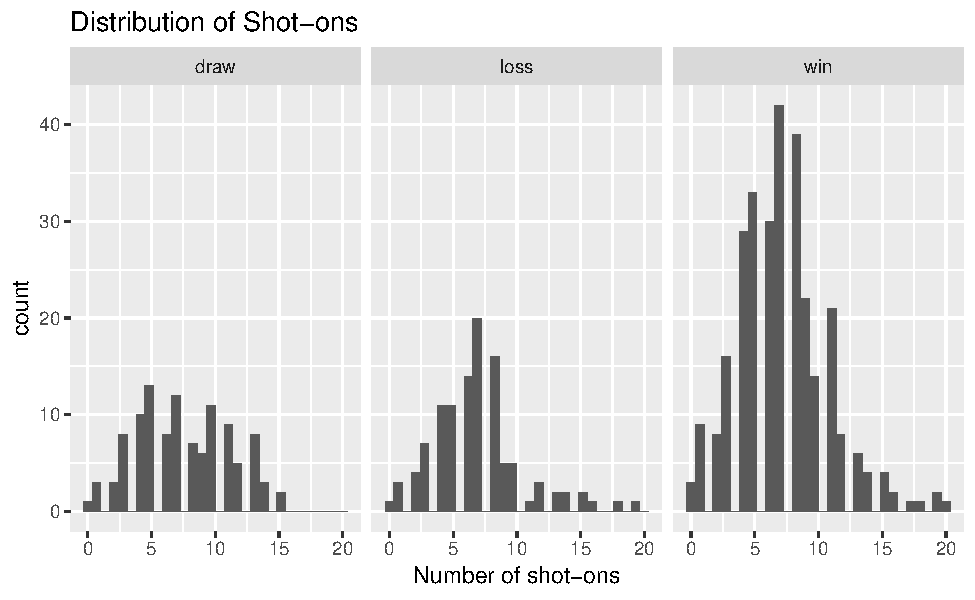
\includegraphics{demo_files/figure-latex/plot-team_shoton-1.pdf}

\subsection{\texorpdfstring{Output Variable -
\texttt{result}}{Output Variable - result}}\label{output-variable---result}

We show the counts of the 3 results: draw, loss, win.

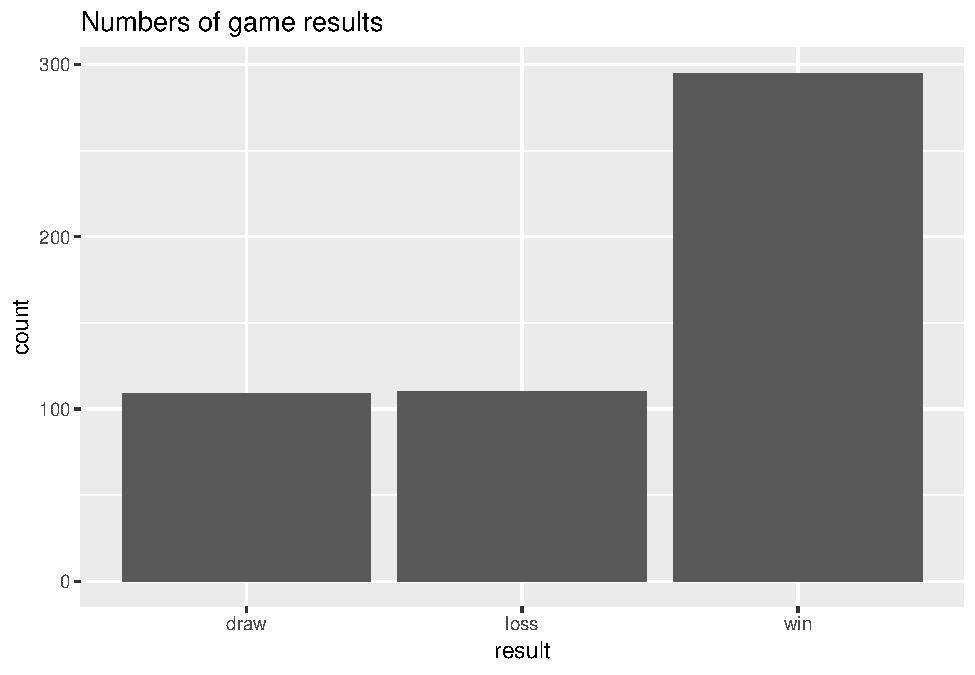
\includegraphics{demo_files/figure-latex/unnamed-chunk-2-1.pdf}

\chapter{Model}\label{model}

\section{Methodology}\label{methodology}

We use the multinomial logistic regression model for estimation. The
response variable \texttt{result} has 3 levels: win, loss, and draw. We
use

\begin{itemize}
\tightlist
\item
  \texttt{game\_type},
\item
  \texttt{team\_shoton}, \texttt{opponent\_shoton},
  \texttt{team\_shotoff}, \texttt{opponent\_shotoff},
\item
  \texttt{team\_corner}, \texttt{opponent\_corner},
\item
  \texttt{team\_cross}, \texttt{opponent\_cross},
\item
  \texttt{team\_pos}, \texttt{opponent\_pos}
\end{itemize}

as the explanatory variables to predict the results.

To avoid overfitting, we apply the penalized LASSO model with
hyperparameter \texttt{lambda} (\(\lambda\)).

\section{Case 1: Manchester United}\label{case-1-manchester-united}

In this section, we focus on building the estimation model for
\textbf{Manchester United}.

\subsection{Model Result}\label{model-result}

The 10-fold cross validation from LASSO algorithm shows that

\[ \text{score}(\text{draw}) = 0.0086 * \text{away game} \]
\[ \text{score}(\text{loss}) = 0.0052 * \text{team crosses} - 0.0090 * \text{opponent crosses} \]

\[ \text{score}(\text{win}) = -0.040 * \text{team fouls} - 0.0046 * \text{team crosses} + 0.036 * \text{team possession} - 0.5123 * \text{away game} \]

Using penalized hyperparameter \(\lambda= 0.07\), we get the that the
model is 51.4\% correct.

\section{Case 2: Liverpool}\label{case-2-liverpool}

In this section, we focus on building the estimation model for
\textbf{Liverpool}.

\subsection{Model Result}\label{model-result-1}

The 10-fold cross validation from LASSO algorithm shows that

\[ \text{score}(\text{draw}) = 0 \]
\[ \text{score}(\text{loss}) = -0.001 * \text{team cross} + 0.254 * \text{away game} \]

\[ \text{score}(\text{win}) = -0.017 * \text{team cross} + 0.018 * \text{team possession} \]

Using penalized hyperparameter \(\lambda=\) 0.0967407, we get the that
the model is 51.4\% correct.

\bibliography{book.bib,packages.bib}


\end{document}
